En esta sección se describe el diseño y desarrollo de cada etapa del proyecto desde 2015 hasta la actualidad. Dichos avances pueden encontrarse en \cite{Proyecciones_0417} y \cite{Proyecciones_1017}, publicaciones realizadas durante el trabajo en los Proyectos de Investigación y Desarrollo dirigidos por el Ing. Sebastián Verrastro:
\begin{itemize}
\item Diseño y testing de circuitos integrados de bajo consumo para aplicaciones médicas implantables.
\item Investigación y desarrollo de un circuito 
integrado transceptor por radio frecuencia, 
pasivo y de bajo consumo.
\end{itemize}

\subsection{Modulador} \label{subsec:modulador}
\subsubsection{Diseño del modulador de carga}
La comunicación desde la PICC hacia el PCD se lleva a cabo mediante variaciones en la carga del primer dispositivo, lo que genera, a su vez, variaciones de tensión en el segundo. Esta forma de comunicación es conocida como modulación de carga. Las variaciones de tensión dependen, principalmente, del nivel de acoplamiento existente entre ambos dispositivos, de la topología del modulador escogida y de los valores de componentes usados en la topología elegida.
A través de la modulación de carga, se generan bandas laterales de modulación en el espectro (Figura \ref{fig:Mod_carg}). Si se generan variaciones con una frecuencia alta $f_s$, se crean dos líneas espectrales a una distancia $\pm f_s$ alrededor de la frecuencia de transmisión del PCD.
Las variaciones de tensión que se observan en el PCD son características propias de la modulación por desplazamiento de amplitud que se genera a través de las variaciones de la carga en el PICC. La ASK se caracteriza por desarrollarse a través de la variación de la señal portadora entre dos valores de amplitud, es decir, entre dos estados, a una frecuencia $f_s$. La modulación ASK tiene características similares a la muy conocida modulación AM (modulación de amplitud). Como esta última, la ASK es lineal, sencilla de implementar y la reconstrucción de los datos enviados es relativamente simple.

\begin{figure}[H]
\centering
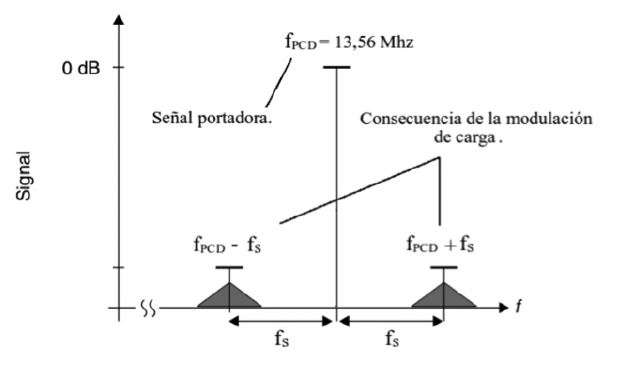
\includegraphics[scale=0.5]{Antecedentes/Modulacion_Carga.JPG}
\caption{Modulación de carga.}
\label{fig:Mod_carg}
\end{figure}


Los moduladores constan de dos transistores
NMOS que se abren y se cierran dependiendo
del valor de tensión que se aplica en la compuerta
de estos. Como se mencionó anteriormente,
la modulación en amplitud maneja dos
estados de tensión, entonces, los transistores
estarán al corte o conduciendo, provocando
una conmutación de carga en paralelo al circuito
resonante.

\begin{figure}[H]
\centering
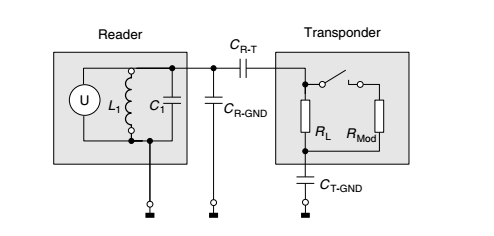
\includegraphics[scale=0.5]{Antecedentes/Modulador_Equiv.png}
\caption{Equivalente del modulador de carga.}
\label{fig:Mod_equ}
\end{figure}

\subsubsection{Modulador Capacitivo}
Analizando las distintas formas de realizar la
modulación de carga, se tomó como primer
circuito a analizar una topología de modulación
capacitiva presentada en la Figura \ref{fig:Mod_carg_cap}. El
funcionamiento de este módulo consta del
agregado (en uno de los estados de $V_Data$) de
capacitores en paralelo al circuito resonante
del PICC, mientras que, en el otro nivel lógico,
el circuito resonante no se ve afectado. Esta
variabilidad de capacidad provoca una mínima
desintonía entre los dispositivos, lo cual influye
en la transferencia de energía entre estos y se
observa como una variación en la tensión observada
en la antena del PCD.
Se realizó, inicialmente, el análisis del comportamiento
del modulador con el equivalente
en pequeña señal de los transistores debido a
que se manejó la posibilidad de que las capacidades
parásitas de estos afecten al circuito
modulador. Finalmente, se corroboró que estas
capacidades no afectan el funcionamiento
del módulo y se realizaron simulaciones para
obtener los valores correctos de $C_1$ y $C_2$ para
realizar una modulación con el mayor índice
de modulación posible. En las simulaciones se
tuvieron en cuenta los valores posibles de integración
para la tecnología. Vale aclarar que, 
a la hora de la integración, los capacitores
ocupan mucha área de silicio por lo que esto
acota los valores de capacidad con los cuales
disponemos para realizar el módulo a valores
menores o alrededor a la decena de pico faradios.
Con los valores de capacidad posibles ya
detectados, se hicieron análisis en frecuencia
para poder observar la “desintonía” que genera
esta topología para lograr la modulación.

\begin{figure}[H]
\centering
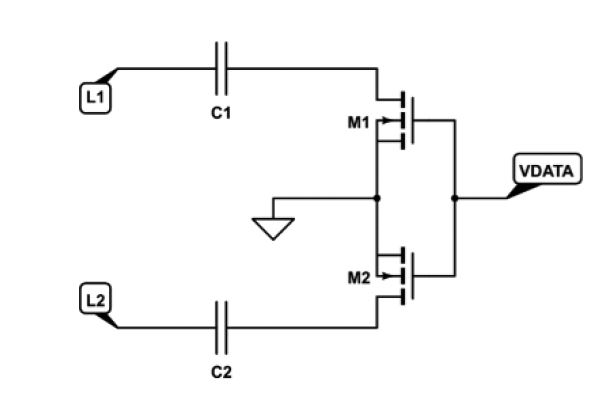
\includegraphics[scale=0.5]{Antecedentes/Modulacion_Carga_Cap.JPG}
\caption{Modulador de carga capacitivo.}
\label{fig:Mod_carg_cap}
\end{figure}

\subsubsection{Modulador óhmico con sólo transistores}
Buscando un mayor índice de modulación (en
este aspecto el modulador capacitivo es débil)
se analizó una topología de modulación óhmica,
en la cual se utiliza la resistencia de salida
propia de los NMOS (Figura \ref{fig:Mod_carg_trans}). 
Al ser
una impedancia baja, cuando se encuentra en
paralelo al circuito resonante y a la carga que
conforman los demás módulos que se encuentran
conectados a este circuito, la impedancia
del conjunto baja considerablemente. Si se varía 
la puesta en paralelo de la impedancia de
salida de los NMOS a la frecuencia $f_s$, se obtiene
una modulación de carga.
A través de la simulación de la topología de
la Figura \ref{fig:Mod_carg_trans}, se observó lo buscado: un índice
de modulación considerablemente mayor al
obtenido anteriormente. En el análisis enfocado
hacia los transistores y su comportamiento
durante la modulación, se detectaron picos
de corriente (Figura \ref{fig:Picos_Cor}), en el drain
de cada uno de los transistores, que podrían
afectar a estos dispositivos luego de un uso
considerable de estos. Estos picos se generan
debido a que, en las simulaciones, los tiempos
de rise (subida) y fall (bajada) de la señal
$V_Data$ son de valores muy pequeños. Si bien
en el uso empírico de los dispositivos estos
valores suelen ser mayores, lo que provocaría
disminución en los picos nombrados, se procedió
a buscar un margen de seguridad en el circuito.
\begin{figure}[H]
\centering
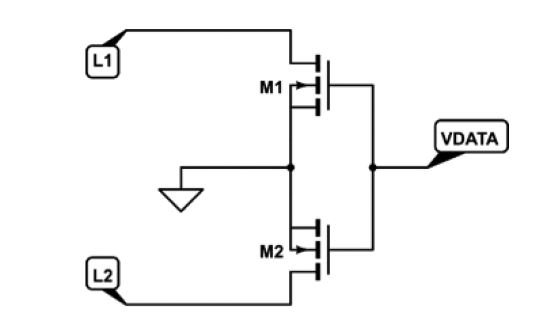
\includegraphics[scale=0.5]{Antecedentes/Modulacion_Carga_Trans.JPG}
\caption{Modulador de carga óhmico.}
\label{fig:Mod_carg_trans}
\end{figure}

\begin{figure}[H]
\centering
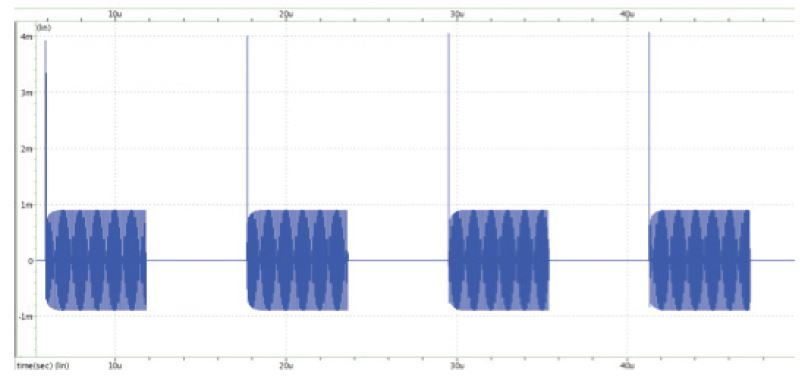
\includegraphics[scale=0.5]{Antecedentes/Picos_Corriente.JPG}
\caption{Corriente en el drain del NMOS M2 en la topología sin capacitores ni resistores.}
\label{fig:Picos_Cor}
\end{figure}


\subsubsection{Modulador óhmico con resistores}
Buscando la protección de los transistores
ante picos de corrientes inesperados se
modificó la topología de la Figura 8 mediante
el uso de dos resistores que protejan los
drenajes de los NMOS pero que, a su vez, no
disminuyan considerablemente la modulación
obtenida con la topología anterior. El nuevo
circuito quedó conformado como se muestra
en la Figura \ref{fig:Mod_carg_res}.
Para encontrar el valor de capacidades en la
topología de la Figura \ref{fig:Mod_carg_cap} se habían tenido en
cuenta ciertos parámetros deseados. Con los
resistores se trabajó de forma similar, pero
enfocando el diseño en otros parámetros. Se
buscaron valores de resistencias que realicen
una protección correcta de los transistores y
que, a su vez, no afecten de forma considerable
al índice de modulación logrado con la
topología de la Figura \ref{fig:Mod_carg_trans}.
Luego de verificar que los picos de corrientes
en los drenajes de los NMOS eran considerablemente
menores a los vistos en la topología
anterior y que la modulación generada en el
circuito resonante del PCD mantenía un buen
índice de modulación, se continuó con los análisis
a esta topología.
Uno de los problemas que pueden surgir en los
circuitos electrónicos son los comportamientos
indeseados debido a variaciones e incertidumbres
en los componentes que componen los
circuitos. Para asegurarse que, ante estas variaciones,
el circuito seguirá funcionando como
se desea, es que se realizan las simulaciones
con el método de Montecarlo. Este método
consiste en realizar un análisis estadístico numérico
analizando el comportamiento del circuito
ante variaciones probabilísticas en sus
componentes. Realizando estas simulaciones
para variaciones de los valores nominales de
los resistores $R_1$ y $R_2$ nos aseguramos que el
circuito mantenga su correcto funcionamiento
en el caso de alteraciones en estos.
Para aumentar nuestro margen de funcionabilidad,
el circuito se sometió a simulaciones
mediante corners (extremos del proceso) que
contienen las posibles variaciones en las características
de los transistores provocadas por el
proceso de fabricación del CI.

\begin{figure}[H]
\centering
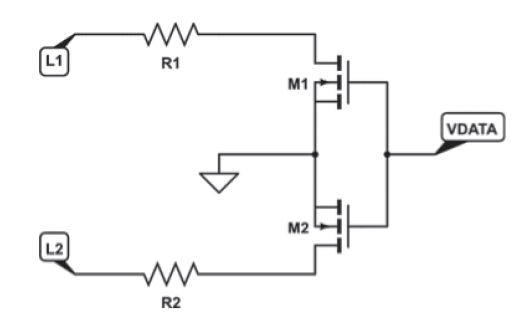
\includegraphics[scale=0.5]{Antecedentes/Modulacion_Carga_Res.JPG}
\caption{Modulador de carga óhmico con resistores.}
\label{fig:Mod_carg_res}
\end{figure}

A continuación, en la fig. \ref{fig:prof_moduladores}, se muestra uno de los factores usados para comparar las distintas topologías.

\begin{figure}[H]
 \centering
  \subfloat[Modulador capacitivo.]{
   \label{f:prof_cap}
    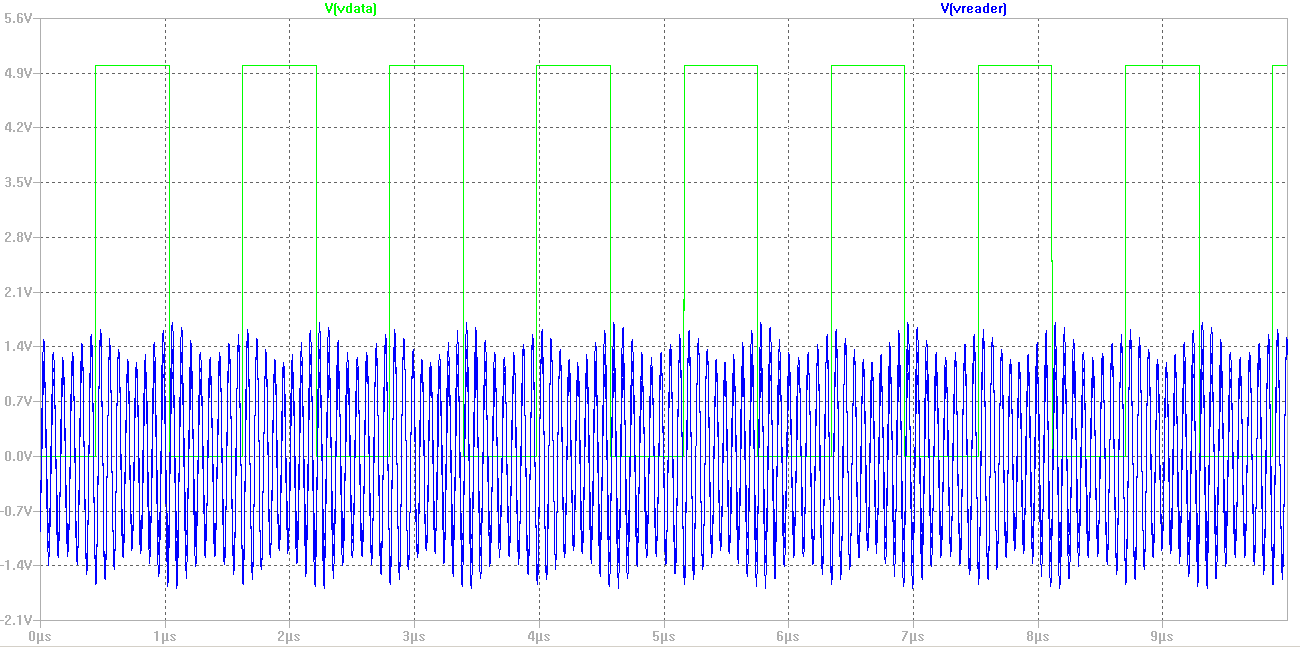
\includegraphics[width=0.5\textwidth]{Antecedentes/Load_Modulation_Cap_Vreader.png}}
  \subfloat[Modulador óhmico sin resistores.]{
   \label{f:prof_trans}
    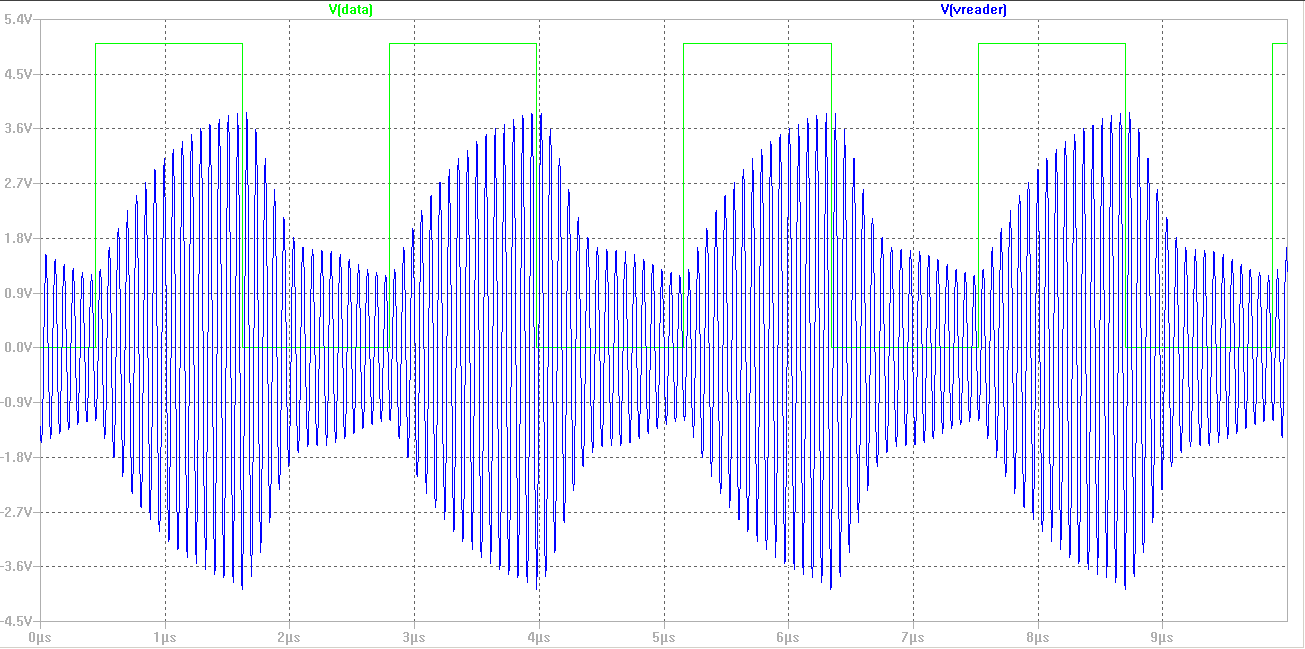
\includegraphics[width=0.5\textwidth]{Antecedentes/Load_Modulation_2_VReader.png}}
    \newline
  \subfloat[Modulador óhmico con resistores.]{
   \label{f:prof_res}
    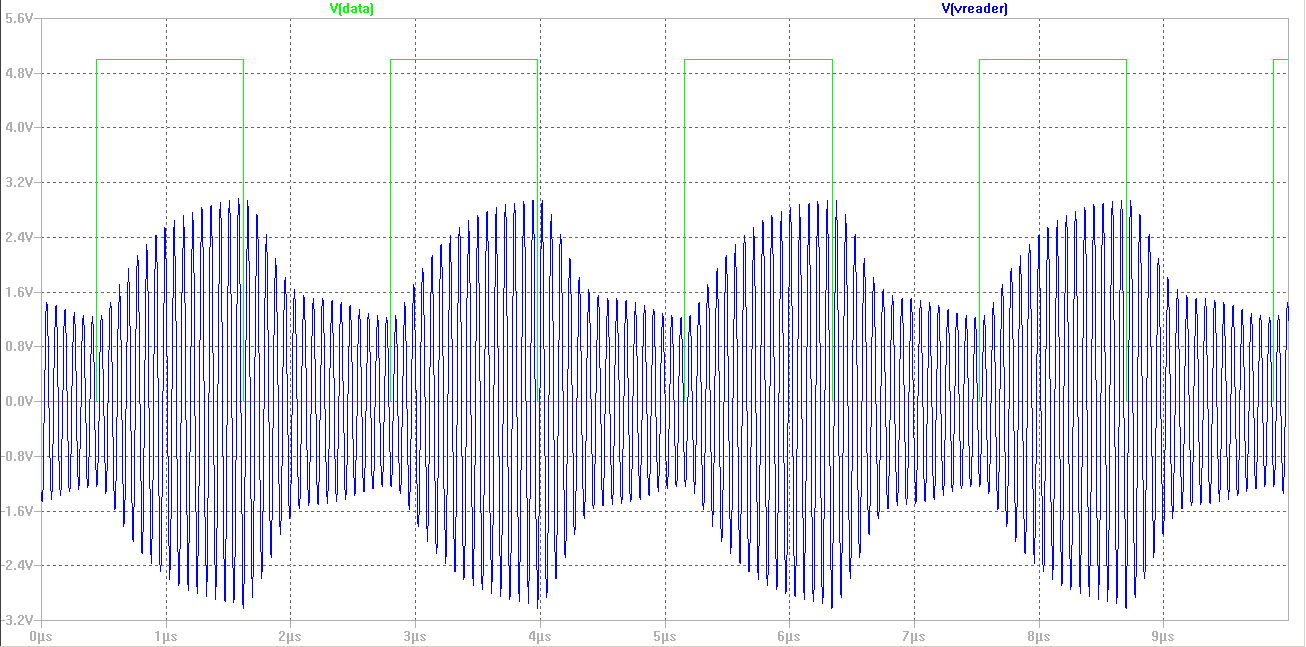
\includegraphics[width=0.5\textwidth]{Antecedentes/LoadModulation1_Reader.png}}
 \caption{Profundidad de modulación de las diferentes topologías de modulador.}
 \label{fig:prof_moduladores}
\end{figure}


\subsection{Demodulador} \label{subsec:demodulador}
La comunicación desde el PCD al PICC se lleva a cabo mediante una
modulación ASK al 100\% con una codificación Miller Modificado
(Norma ISO14443 Tipo A). La modulación ASK
tiene como característica la variación de la señal
portadoras entre dos valores definidos. En
una modulación ASK al 100\%, la señal variará
entre un nivel de tensión mayor a cero y 0V
(cero Volt).
Se utilizaron varias topologías de demoduladores.
En la primer topología, la demodulación de la señal recibida en el
PICC, se llevó a cabo a través de varias etapas \ref{fig:Demo}. En primer lugar, se realizó la rectificación
de la señal y la detección de envolvente.
En una segunda etapa, se filtró la señal obtenida
en la etapa anterior para evitar errores en
la próxima fase de tratamiento de señal debido
a variaciones de alta frecuencia sobre la señal
envolvente. En la última parte, se ingresó la
señal ya filtrada a un Schmitt trigger \cite{schmitt} para obtener, a la salida, la señal
que representa los datos enviados por el PCD.
\begin{figure}[H]
\centering
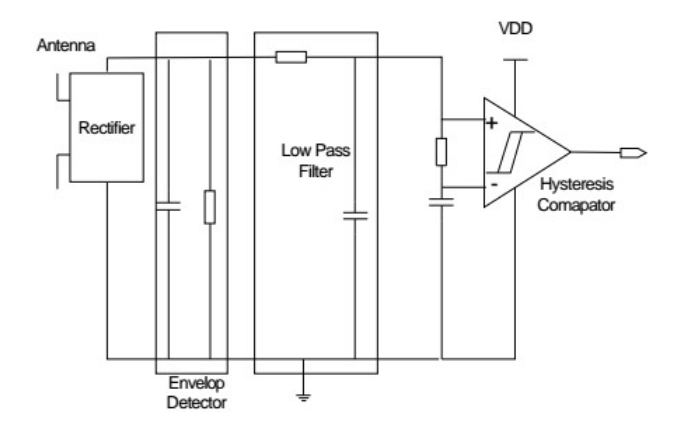
\includegraphics[scale=0.5]{Antecedentes/Demodulador.png}
\caption{Estructura básica de un demodulador \cite{RFID_Tuto}.}
\label{fig:Demo}
\end{figure}
La segunda topología utilizada (fig \ref{fig:Demod2}), además de estar conformada
por el Schmitt trigger y un filtro pasabajos,
posee en el diseño, un comparador y una entrada
de habilitación. Ésta tiene la ventaja de
poder ajustar el nivel del comparador externamente.
La desventaja es que el amplificador
operacional diseñado tiene un tiempo de
respuesta (Slew Rate) mucho mayor que el
Schmitt trigger.

\begin{figure}[H]
\centering
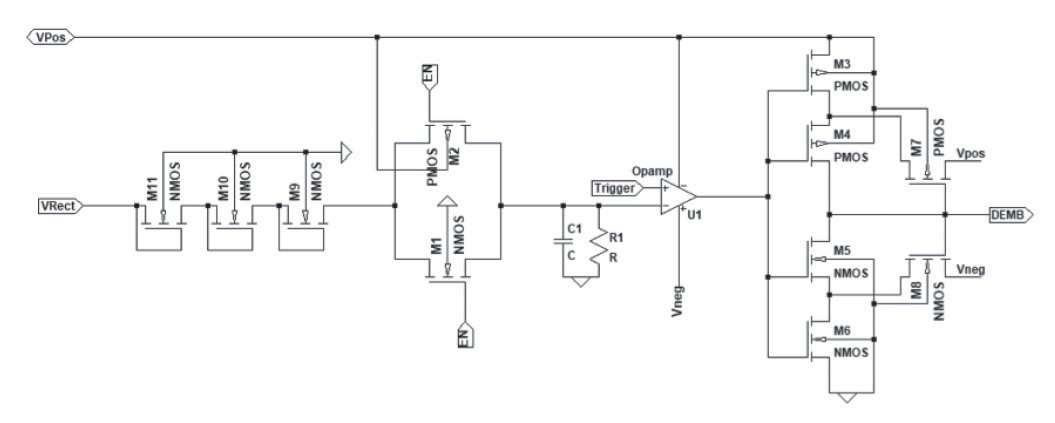
\includegraphics[scale=0.5]{Antecedentes/Demod2.PNG}
\caption{Esquemático de la segunda topología de demodulador utilizada.}
\label{fig:Demod2}
\end{figure}

\subsubsection{Rectificador y detector de envolvente}
En esta etapa se usó una topología típica de
un demodulador de AM (amplitud modulada),
la cual se ve en la Fig.\ref{fig:Detect} y se caracteriza
por ser un circuito simple, compuesto por un
rectificador y un detector (Resistor y Capacitor
en paralelo).
\begin{figure}[H]
\centering
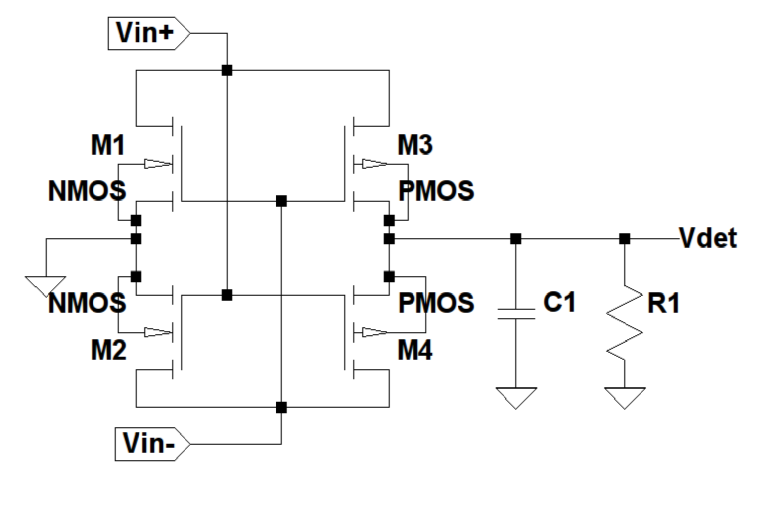
\includegraphics[scale=0.3]{Antecedentes/Detect_RC.png}
\caption{Rectificador y detector de envolvente.}
\label{fig:Detect}
\end{figure}
A continuación, se realizó el análisis matemático
de la topología para obtener los valores de
componentes que optimizan el funcionamiento
del circuito. Para un análisis más sencillo, se
optó por tomar como rectificador a un diodo.
Teniendo en cuenta que el detector de envolvente
se compone de un resistor y un capacitor, éste presenta una constante de tiempo $\tau = RC$.
Considerando también que se tiene una señal
portadora con una frecuencia igual a $f_c =
13,56 MHz$, el capacitor se descarga, entre
cada pico de portadora, siguiendo la siguiente
ecuación:
$$V'_{pico} = V_{pico}e^{-\frac{t}{\tau}}$$
Donde $T = \frac{1}{fc}$. Si tomamos $T << \tau$, entonces:
$$\bigtriangledown V \simeq V{pico}\frac{T}{\tau} = \frac{V_{pico}}{f_c \tau}$$

Cuando la señal está modulada en ASK, su
tensión pasa, de un valor de tensión definido
a un valor mucho menor (cero Volts en nuestro
caso). La caída de tensión en el detector
de envolvente, desde un valor a otro, se ve en la siguiente ecuación:
$$V_{caida} = V_{pico}e^{-\frac{t}{\tau}}$$

Desde la ecuación anterior, puede analizarse
el comportamiento del circuito detector ante el
cambio de tensión mencionado. Dependiendo
del \tau del RC, éste será más o menos sensible al
cambio de tensión.
Buscando, en la práctica, una buena relación
en la respuesta del circuito detector ante el
cambio de tensión a la frecuencia modulante
y ante el ripple a la frecuencia portadora, se
toma un \tau dentro del intervalo de la ecuación
siguiente:
$$\frac{1}{f_c} << \tau << \frac{1}{f_m}$$
Entonces, teniendo 13,56 MHz como $f_c$ (frecuencia
de portadora) y 106 kHz como $f_m$ (frecuencia
modulante) se escogieron los siguientes
valores de componente:
$$R = 5 k\Omega ; C = 30 pF$$
Quedándonos la siguiente relación entre frecuencias
y \tau:
$$\frac{1}{13.56MHz}<<1.5.10^{-7}s<<\frac{1}{106kHz}$$

\begin{figure}[H]
\centering
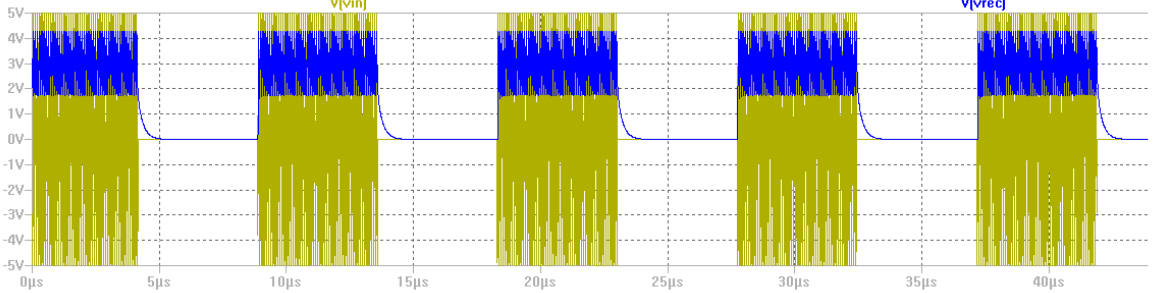
\includegraphics[scale=0.3]{Antecedentes/Sim_Detect.png}
\caption{Señal de entrada y señal de salida del detector de envolvente \tau = 0,15\mu S.}
\label{fig:Sim_detect}
\end{figure}

\subsubsection{Filtro pasa bajos}
Una vez que, la señal modulada que llega al
PICC, pasa por el detector de envolvente, ésta,
queda con un ripple a la frecuencia de la portadora.
Para evitar que en la siguiente etapa se
produzcan fallas debido a variaciones de tensión
no deseadas, la señal de salida del detector,
pasa por un filtro RC (pasa bajos simple) cuyo
fin es mitigar las ondulaciones a 13,56 MHz.
La frecuencia de corte del filtro deberá estar por
debajo de la frecuencia de portadora, para así
filtrarla y por encima de la frecuencia modulante,
para no afectar la envolvente. Entonces:
$$\frac{1}{106kHz}<<f_c<<\frac{1}{13.56MHz}$$
$$f_c = \frac{1}{2\pi RC} \approx 3.2MHz$$
$$R = 10 k\Omega ; C = 6 pF$$

\begin{figure}[H]
\centering
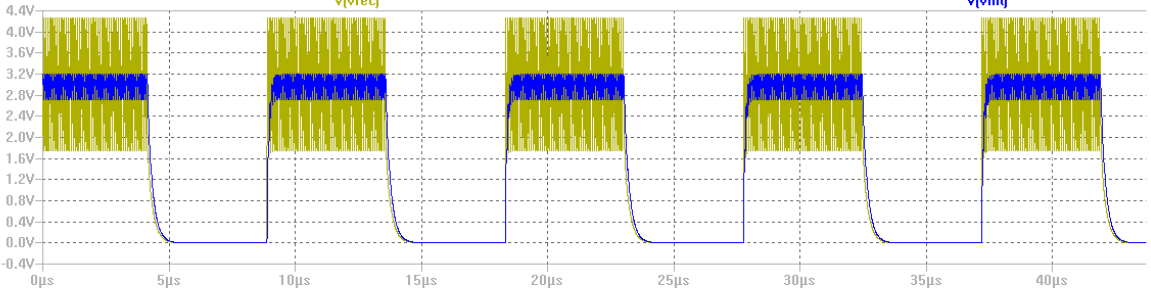
\includegraphics[scale=0.3]{Antecedentes/Sim_RC.png}
\caption{Filtrado del riple de 13.56MHz con filtro RC.}
\label{fig:Sim_RC}
\end{figure}

\subsubsection{Schmitt trigger}
Dado que la señal de salida del demodulador
ingresará luego a un sistema digital, ésta debe
estar libre de ruido y distorsiones para evitar
errores en la información y, por lo tanto, en el
sistema encargado del manejo de la información.
Una forma de digitalizar una señal, eliminando
las perturbaciones que trae, es a través
de un Schmitt trigger.
Este tipo de disparador se caracteriza por su
naturaleza biestable y por el uso de una histéresis
que gobierna los cambios de estados. La
topología escogida es la de un inversor CMOS
de doble transistor con la adición de un par de
transistores que son los que definen los puntos
de cambio de estado en la histéresis.
Esta topología, cuenta con la ventaja de poder
escoger los puntos de disparo del sistema eligiendo
la relación de aspecto de los transistores que la conforman. 
Las relaciones entre el ancho
y el largo del canal de los transistores, tienen
efecto en la histéresis del disparador.

\begin{figure}[H]
\centering
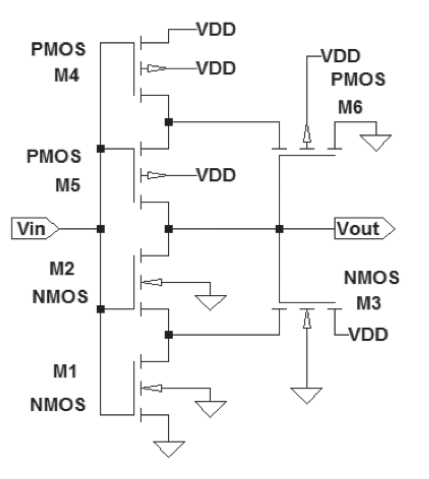
\includegraphics[scale=0.5]{Antecedentes/Schmitt_Trigger.PNG}
\caption{Schmitt Trigger CMOS.}
\label{fig:Schmit}
\end{figure}

Cuando en la entrada del circuito (Fig. \ref{fig:Schmit}) hay
0 V, los transistores $M_4$ y $M_5$, estarán conduciendo,
mientras que el $M_1$ y el $M_2$, estarán en
corte. Con esa condición, la salida estará en alto
($V_{out} = V_{DD}$). Cuando la tensión de entrada comience
a subir y alcance la tensión de umbral
del transistor $M_1$, éste comenzará a conducir,
pero el $M_2$ se mantendrá apagado. El $M_1$ tenderá
a hacer bajar el nodo entre éste y el $M_2$ a
GND, mientras que, el $M_3$, que tiene $V_{DD}$ en su
gate, hará tender el nodo hacia $V_{DD}$. Cuando la
señal de entrada supere la tensión umbral del
$M_2$, entonces, éste comenzará a conducir y la
salida tendrá 0V de tensión, denominando la
tensión de entrada que dispara la salida al nivel
bajo como $V_{IH}$ (tensión límite que se admite
como uno lógico).
Algo similar ocurre con la rama superior del inversor
cuando la tensión de entrada comienza a
disminuir. Los transistores $M_4$ y $M_6$ harán tender
el nodo hacía VDD y GND respectivamente,
hasta que el $M_5$ comience a conducir y la salida
pase al estado alto, denominando, entonces, la
tensión de entrada que dispara la salida al nivel
alto como $V_{IL}$ (tensión límite que se admite
como cero lógico).
Partiendo del análisis en condiciones de saturación
de los transistores $M_1$ y $M_3$ se llegó a la
expresión de la $V_{IH}$ en función de las relaciones
de aspecto de dichos transistores:
$$I_{DM3} = \frac{\beta _3}{2(V_{GS}-V_{TH3})^2}$$
Siendo:
$$\beta = \mu _n C_{ox} (\frac{W}{L})^2 $$
Donde $\mu _n$ e la movilidad de los electrones en el silicio, $C_ox$ es la capacidad del Óxido, W el ancho de la compuerta
del transistor y L el largo de la compuerta del transistor.

Desarrollando y teniendo en cuenta que:
$$V_{TH2} = V_{TH2};  I_{DM3} = I_{DM1}$$
Puede llegarse a la siguiente expresión:
$$V_{IH}= \frac{V_{DD}+V_{VTH1}\sqrt[]{\frac{\beta _1}{\beta _3}}}{1+\sqrt[]{\frac{\beta _1}{\beta _3}}}$$

Haciéndose un análisis similar, pero en condiciones
de saturación para los transistores $M_6$ y $M_4$, se
llega a la expresión de VIL:
$$I_{DM6} = \frac{\beta _6}{2(V_{SG}-|V_{TH6}|)^2}$$

Desarrollando y teniendo en cuenta que:
$$V_{TH5} = V_{TH6};  I_{DM4} = I_{DM6}$$
Puede llegarse a la siguiente ecuación:
$$V_{IL}= \frac{\sqrt[]{(\frac{\beta _4}{\beta _6})(V_{DD}-|V_{TH4}|)}}{1+\sqrt[]{\frac{\beta _4}{\beta _6}}}$$
Una vez encontradas las expresiones de $V_{IL}$ y
$V_{IH}$, se buscó una relación entre los tamaños de
los transistores, para lograr un óptimo funcionamiento
del circuito, evitando errores por ruido
de alta frecuencia y distorsiones en la señal de
entrada.

\begin{figure}[H]
\centering
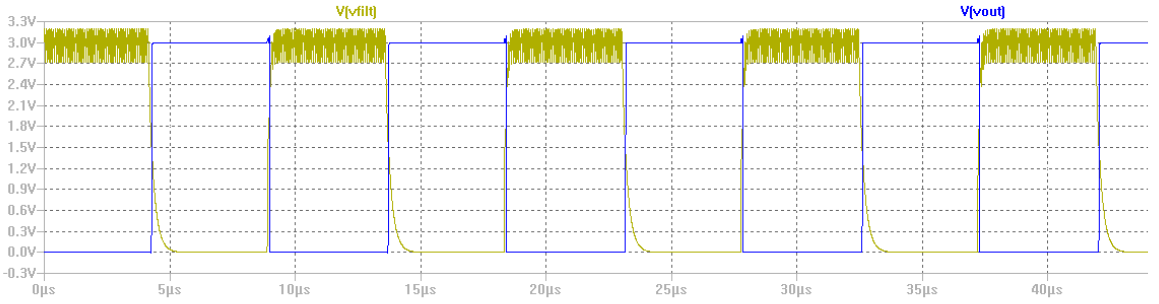
\includegraphics[scale=0.3]{Antecedentes/Sim_Schmit.png}
\caption{Tensión de entrada y de la salida del Schmitt Trigger.}
\label{fig:Sim_Schmit}
\end{figure}

Como resultado de todas las etapas mencionadas anteriormente, se obtuvo un demodulador que opera según la fig. \ref{fig:Sim_demo}.

\begin{figure}[H]
\centering
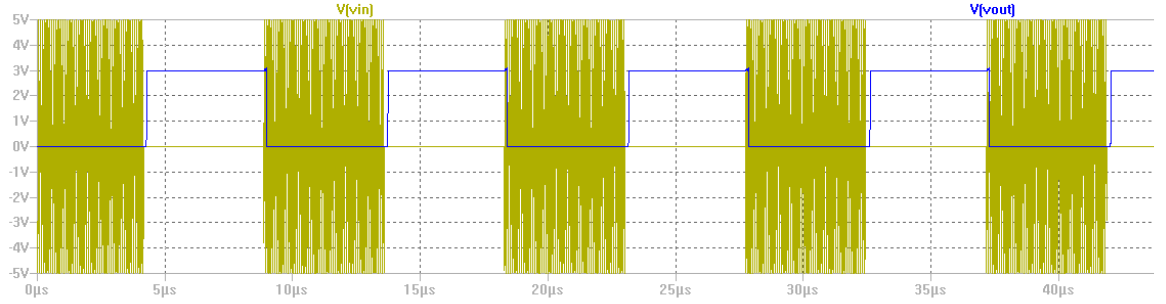
\includegraphics[scale=0.3]{Antecedentes/Sim_Demo.png}
\caption{Tensión de entrada y de la salida del demodulador.}
\label{fig:Sim_demo}
\end{figure}



\subsection{Limitador (Shunt)} \label{subsec:limit}

Se eligieron dos topologías de limitador Shunt, la primera topología se basó en el de Zheng Zhu \cite{shunt1}, y la segunda topología en Napong Panitantu \cite{shunt2}.

Al final se implementó en el desarrollo final la topología de Napong, ya que los resultados fueron más óptimos \cite{Proyecciones_1017}. En la figura \ref{fig:shunt2} se muestra la topología.

\begin{figure}[H]
\centering
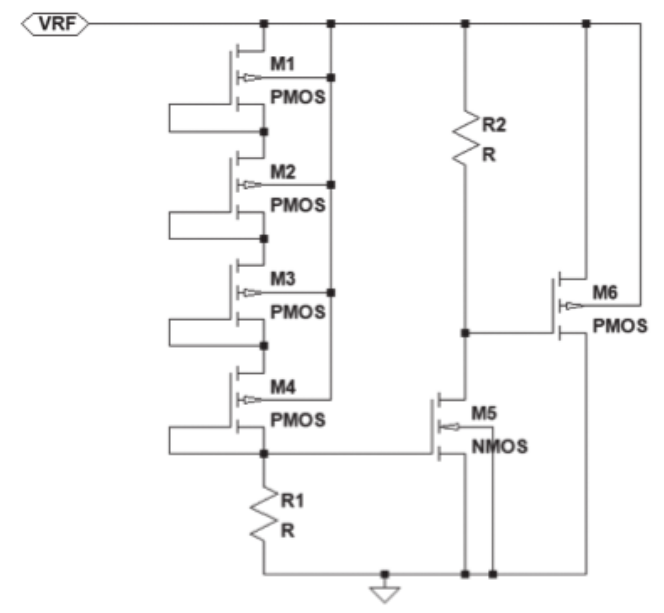
\includegraphics[width=0.4\linewidth]{circuitos/Shunt_2.png}
\caption{Limitador de potencia - Shunt}
\label{fig:shunt2}
\end{figure}

Siendo:

$$Vgs_{6} > Vth_{p}$$

lo que ocurre cuando el transistor M5 se encuentra en saturación. Dicha situación se logra cuando la tensión sobre el gate del transistor M5 es:

$$Vgs_{6} = Vrf - Vds_{5}$$
$$Vgs_{5} > (Vrf - Vgs_{1} + Vgs_{2} + Vgs_{3} + Vgs_{4}) $$

En función de esto se diseñó la topología para que a partir de los 6 V (para el caso de ONC5) comience a operar el transistor M6. En las figuras \ref{fig:shunt_500} y \ref{fig:shunt_500} se observan resultados obtenidos en la simulación de este módulo.